% Options for packages loaded elsewhere
\PassOptionsToPackage{unicode}{hyperref}
\PassOptionsToPackage{hyphens}{url}
\PassOptionsToPackage{dvipsnames,svgnames,x11names}{xcolor}
%
\documentclass[
  11pt,
  a4paper,
  DIV=11,
  numbers=noendperiod]{scrartcl}

\usepackage{amsmath,amssymb}
\usepackage{iftex}
\ifPDFTeX
  \usepackage[T1]{fontenc}
  \usepackage[utf8]{inputenc}
  \usepackage{textcomp} % provide euro and other symbols
\else % if luatex or xetex
  \usepackage{unicode-math}
  \defaultfontfeatures{Scale=MatchLowercase}
  \defaultfontfeatures[\rmfamily]{Ligatures=TeX,Scale=1}
\fi
\usepackage{lmodern}
\ifPDFTeX\else  
    % xetex/luatex font selection
    \setmainfont[]{Avenir Next}
\fi
% Use upquote if available, for straight quotes in verbatim environments
\IfFileExists{upquote.sty}{\usepackage{upquote}}{}
\IfFileExists{microtype.sty}{% use microtype if available
  \usepackage[]{microtype}
  \UseMicrotypeSet[protrusion]{basicmath} % disable protrusion for tt fonts
}{}
\makeatletter
\@ifundefined{KOMAClassName}{% if non-KOMA class
  \IfFileExists{parskip.sty}{%
    \usepackage{parskip}
  }{% else
    \setlength{\parindent}{0pt}
    \setlength{\parskip}{6pt plus 2pt minus 1pt}}
}{% if KOMA class
  \KOMAoptions{parskip=half}}
\makeatother
\usepackage{xcolor}
\setlength{\emergencystretch}{3em} % prevent overfull lines
\setcounter{secnumdepth}{-\maxdimen} % remove section numbering
% Make \paragraph and \subparagraph free-standing
\makeatletter
\ifx\paragraph\undefined\else
  \let\oldparagraph\paragraph
  \renewcommand{\paragraph}{
    \@ifstar
      \xxxParagraphStar
      \xxxParagraphNoStar
  }
  \newcommand{\xxxParagraphStar}[1]{\oldparagraph*{#1}\mbox{}}
  \newcommand{\xxxParagraphNoStar}[1]{\oldparagraph{#1}\mbox{}}
\fi
\ifx\subparagraph\undefined\else
  \let\oldsubparagraph\subparagraph
  \renewcommand{\subparagraph}{
    \@ifstar
      \xxxSubParagraphStar
      \xxxSubParagraphNoStar
  }
  \newcommand{\xxxSubParagraphStar}[1]{\oldsubparagraph*{#1}\mbox{}}
  \newcommand{\xxxSubParagraphNoStar}[1]{\oldsubparagraph{#1}\mbox{}}
\fi
\makeatother

\usepackage{color}
\usepackage{fancyvrb}
\newcommand{\VerbBar}{|}
\newcommand{\VERB}{\Verb[commandchars=\\\{\}]}
\DefineVerbatimEnvironment{Highlighting}{Verbatim}{commandchars=\\\{\}}
% Add ',fontsize=\small' for more characters per line
\usepackage{framed}
\definecolor{shadecolor}{RGB}{241,243,245}
\newenvironment{Shaded}{\begin{snugshade}}{\end{snugshade}}
\newcommand{\AlertTok}[1]{\textcolor[rgb]{0.68,0.00,0.00}{#1}}
\newcommand{\AnnotationTok}[1]{\textcolor[rgb]{0.37,0.37,0.37}{#1}}
\newcommand{\AttributeTok}[1]{\textcolor[rgb]{0.40,0.45,0.13}{#1}}
\newcommand{\BaseNTok}[1]{\textcolor[rgb]{0.68,0.00,0.00}{#1}}
\newcommand{\BuiltInTok}[1]{\textcolor[rgb]{0.00,0.23,0.31}{#1}}
\newcommand{\CharTok}[1]{\textcolor[rgb]{0.13,0.47,0.30}{#1}}
\newcommand{\CommentTok}[1]{\textcolor[rgb]{0.37,0.37,0.37}{#1}}
\newcommand{\CommentVarTok}[1]{\textcolor[rgb]{0.37,0.37,0.37}{\textit{#1}}}
\newcommand{\ConstantTok}[1]{\textcolor[rgb]{0.56,0.35,0.01}{#1}}
\newcommand{\ControlFlowTok}[1]{\textcolor[rgb]{0.00,0.23,0.31}{\textbf{#1}}}
\newcommand{\DataTypeTok}[1]{\textcolor[rgb]{0.68,0.00,0.00}{#1}}
\newcommand{\DecValTok}[1]{\textcolor[rgb]{0.68,0.00,0.00}{#1}}
\newcommand{\DocumentationTok}[1]{\textcolor[rgb]{0.37,0.37,0.37}{\textit{#1}}}
\newcommand{\ErrorTok}[1]{\textcolor[rgb]{0.68,0.00,0.00}{#1}}
\newcommand{\ExtensionTok}[1]{\textcolor[rgb]{0.00,0.23,0.31}{#1}}
\newcommand{\FloatTok}[1]{\textcolor[rgb]{0.68,0.00,0.00}{#1}}
\newcommand{\FunctionTok}[1]{\textcolor[rgb]{0.28,0.35,0.67}{#1}}
\newcommand{\ImportTok}[1]{\textcolor[rgb]{0.00,0.46,0.62}{#1}}
\newcommand{\InformationTok}[1]{\textcolor[rgb]{0.37,0.37,0.37}{#1}}
\newcommand{\KeywordTok}[1]{\textcolor[rgb]{0.00,0.23,0.31}{\textbf{#1}}}
\newcommand{\NormalTok}[1]{\textcolor[rgb]{0.00,0.23,0.31}{#1}}
\newcommand{\OperatorTok}[1]{\textcolor[rgb]{0.37,0.37,0.37}{#1}}
\newcommand{\OtherTok}[1]{\textcolor[rgb]{0.00,0.23,0.31}{#1}}
\newcommand{\PreprocessorTok}[1]{\textcolor[rgb]{0.68,0.00,0.00}{#1}}
\newcommand{\RegionMarkerTok}[1]{\textcolor[rgb]{0.00,0.23,0.31}{#1}}
\newcommand{\SpecialCharTok}[1]{\textcolor[rgb]{0.37,0.37,0.37}{#1}}
\newcommand{\SpecialStringTok}[1]{\textcolor[rgb]{0.13,0.47,0.30}{#1}}
\newcommand{\StringTok}[1]{\textcolor[rgb]{0.13,0.47,0.30}{#1}}
\newcommand{\VariableTok}[1]{\textcolor[rgb]{0.07,0.07,0.07}{#1}}
\newcommand{\VerbatimStringTok}[1]{\textcolor[rgb]{0.13,0.47,0.30}{#1}}
\newcommand{\WarningTok}[1]{\textcolor[rgb]{0.37,0.37,0.37}{\textit{#1}}}

\providecommand{\tightlist}{%
  \setlength{\itemsep}{0pt}\setlength{\parskip}{0pt}}\usepackage{longtable,booktabs,array}
\usepackage{calc} % for calculating minipage widths
% Correct order of tables after \paragraph or \subparagraph
\usepackage{etoolbox}
\makeatletter
\patchcmd\longtable{\par}{\if@noskipsec\mbox{}\fi\par}{}{}
\makeatother
% Allow footnotes in longtable head/foot
\IfFileExists{footnotehyper.sty}{\usepackage{footnotehyper}}{\usepackage{footnote}}
\makesavenoteenv{longtable}
\usepackage{graphicx}
\makeatletter
\newsavebox\pandoc@box
\newcommand*\pandocbounded[1]{% scales image to fit in text height/width
  \sbox\pandoc@box{#1}%
  \Gscale@div\@tempa{\textheight}{\dimexpr\ht\pandoc@box+\dp\pandoc@box\relax}%
  \Gscale@div\@tempb{\linewidth}{\wd\pandoc@box}%
  \ifdim\@tempb\p@<\@tempa\p@\let\@tempa\@tempb\fi% select the smaller of both
  \ifdim\@tempa\p@<\p@\scalebox{\@tempa}{\usebox\pandoc@box}%
  \else\usebox{\pandoc@box}%
  \fi%
}
% Set default figure placement to htbp
\def\fps@figure{htbp}
\makeatother

\usepackage[document]{ragged2e}
\KOMAoption{captions}{tableheading}
\makeatletter
\@ifpackageloaded{caption}{}{\usepackage{caption}}
\AtBeginDocument{%
\ifdefined\contentsname
  \renewcommand*\contentsname{Table of contents}
\else
  \newcommand\contentsname{Table of contents}
\fi
\ifdefined\listfigurename
  \renewcommand*\listfigurename{List of Figures}
\else
  \newcommand\listfigurename{List of Figures}
\fi
\ifdefined\listtablename
  \renewcommand*\listtablename{List of Tables}
\else
  \newcommand\listtablename{List of Tables}
\fi
\ifdefined\figurename
  \renewcommand*\figurename{Figure}
\else
  \newcommand\figurename{Figure}
\fi
\ifdefined\tablename
  \renewcommand*\tablename{Table}
\else
  \newcommand\tablename{Table}
\fi
}
\@ifpackageloaded{float}{}{\usepackage{float}}
\floatstyle{ruled}
\@ifundefined{c@chapter}{\newfloat{codelisting}{h}{lop}}{\newfloat{codelisting}{h}{lop}[chapter]}
\floatname{codelisting}{Listing}
\newcommand*\listoflistings{\listof{codelisting}{List of Listings}}
\makeatother
\makeatletter
\makeatother
\makeatletter
\@ifpackageloaded{caption}{}{\usepackage{caption}}
\@ifpackageloaded{subcaption}{}{\usepackage{subcaption}}
\makeatother

\usepackage{bookmark}

\IfFileExists{xurl.sty}{\usepackage{xurl}}{} % add URL line breaks if available
\urlstyle{same} % disable monospaced font for URLs
\hypersetup{
  pdftitle={I. Datenbanken},
  colorlinks=true,
  linkcolor={blue},
  filecolor={Maroon},
  citecolor={Blue},
  urlcolor={Blue},
  pdfcreator={LaTeX via pandoc}}


\title{I. Datenbanken}
\author{}
\date{}

\begin{document}
\maketitle


\subsubsection{1. Relationale
Datenbanken}\label{relationale-datenbanken}

\begin{itemize}
\item
  Tabellarische Darstellungen sind die Grundstrukturen relationaler
  Datenbanken.
\item
  Begriffe der Theorie: Relation, Relationsbezeichner, Attribut, Tupel,
  Schlüssel, Primärschlüssel.
\item
  Analoge Begriffe in konkreten Datenbanken: Tabelle,
  Tabellenbezeichner, Spalte, Zeile.
\item
  Ein Schlüssel einer Relation ist eine minimale Teilmenge der Attribute
  der Relation, mittels der die einzelnen Tupel der Relation
  unterschieden werden können.
\item
  Der Primärschlüssel ist ein ausgewählter Schlüssel - er wird durch
  Unterstreichen gekennzeichnet.
\end{itemize}

\[ \text{Student} \]

\begin{longtable}[]{@{}lllll@{}}
\toprule\noalign{}
Student-ID & Name & Vorname & Klassen & Adresse \\
\midrule\noalign{}
\endhead
\bottomrule\noalign{}
\endlastfoot
212 & Frei & Emil & KS 2 & Hansastraße 20 \\
134 & Tittel & Dominik & KS 2 & Yorkstraße 23a \\
423 & Klum & Leni & KS 2 & Turnaustraße 43 \\
\end{longtable}

\subsubsection{2. Struktur und Inhalt einer
Relation}\label{struktur-und-inhalt-einer-relation}

Die abstrakte Struktur einer Relation soll von ihrem Inhalt getrennt
werden. Das wird bewerkstelligt mit dem Relationsschema.

\begin{itemize}
\item
  Struktur der Relation Student:

  Student(ID, Name, Vorname, Klasse, Adresse)
\item
  Der Inhalt/Zustand der Relation mit Schema Student ist die
  Relationsinstanz:
\end{itemize}

\[ \text{Student} \]

\begin{longtable}[]{@{}lllll@{}}
\toprule\noalign{}
Student-ID & Name & Vorname & Klasse & Adresse \\
\midrule\noalign{}
\endhead
\bottomrule\noalign{}
\endlastfoot
212 & Frei & Emil & KS 2 & Hansastraße 20 \\
134 & Tittel & Dominik & KS 2 & Yorkstraße 23a \\
423 & Klum & Leni & KS 2 & Turnaustraße 43 \\
\end{longtable}

\begin{itemize}
\tightlist
\item
  Die identifizierende Eigenschaft des Primärschlüssels muss für jede
  Instanz der Relation gewährleistet sein.
\end{itemize}

\subsubsection{3. Beispiel einer
Miniwelt}\label{beispiel-einer-miniwelt}

Student(Student-ID, Name, Vorname, Klasse, Adresse)

Lehrer(Teacher-ID, Vorname, Nachname, Titel)

Fach(Kurzzeichen, Art, Stundenzahl)

\[ \text{Student} \]

\begin{longtable}[]{@{}lllll@{}}
\toprule\noalign{}
Student-ID & Name & Vorname & Klassen & Adresse \\
\midrule\noalign{}
\endhead
\bottomrule\noalign{}
\endlastfoot
212 & Frei & Emil & KS 2 & Hansastraße 20 \\
134 & Tittel & Dominik & KS 2 & Yorkstraße 23a \\
423 & Klum & Leni & KS 2 & Turnaustraße 43 \\
\end{longtable}

\[ \text{Lehrer} \]

\begin{longtable}[]{@{}llll@{}}
\toprule\noalign{}
Lehrer-ID & Vorname & Nachname & Titel \\
\midrule\noalign{}
\endhead
\bottomrule\noalign{}
\endlastfoot
001 & Gerhard & Gauß & Dr \\
002 & Felix & Otto & StD \\
003 & Milena & Tabert & Frau \\
\end{longtable}

\[ \text{Fach} \]

\begin{longtable}[]{@{}lll@{}}
\toprule\noalign{}
Kurzzeichen & Art & Stundenzahl \\
\midrule\noalign{}
\endhead
\bottomrule\noalign{}
\endlastfoot
M & Hauptfach & 5 \\
Inf & Nebenfach & 2 \\
Bio & Nebenfach & 2 \\
\end{longtable}

\subsubsection{4. Datenbankschema und
Datenbankinstanz}\label{datenbankschema-und-datenbankinstanz}

\begin{itemize}
\tightlist
\item
  Die Menge der Relationsschemata einer Miniwelt ergibt das
  (relationale) Datenbankschema der Miniwelt.
\item
  Eine Menge von Instanzen der Relationen eines Datenbankschemas nennen
  wir Datenbankinstanz.
\end{itemize}

Die Elemente einer Datenbankinstanz müssen sich auf denselben Zustand
der betreffenden Miniwelt beziehen.

\subsubsection{5. Modellierung einer
Miniwelt}\label{modellierung-einer-miniwelt}

\paragraph{Objekte und Beziehungen}\label{objekte-und-beziehungen}

\begin{itemize}
\item
  Objekte bilden die elementare Grundlage unserer Betrachtung. Objekte
  werden durch Tupel in Relationen repräsentiert und können somit durch
  Schlüsselwerte identifiziert werden.
\item
  Beziehungen sind über Objekten oder anderen Beziehungen definiert; sie
  entstehen somit durch In-Bezug-Setzen von Objekten.

  Objektreferenzen in Beziehungen: Fremdschlüssel.
\item
  Menge der als relevant betrachteten Objekte und Beziehungen: Miniwelt.
\item
  Objekte und Beziehungen werden getypt. Die Menge der Objekt- und
  Beziehungstypen einer Miniwelt ergibt das konzeptuelle Schema der
  Miniwelt.
\end{itemize}

\paragraph{Beispiel:}\label{beispiel}

Beziehung Teilnahme zwischen Subject und Student

Schlüssel der Relation Participation sind die Primärschlüssel aus den
Relationen Subject und Student: - Student-ID - Kurzzeichen Dieser
Schlüssel wird als Fremdschlüssel bezeichent.

\[ \text{Teilnahme} \]

\begin{longtable}[]{@{}lll@{}}
\toprule\noalign{}
Student-ID & Kurzzeichen & Schuljahr \\
\midrule\noalign{}
\endhead
\bottomrule\noalign{}
\endlastfoot
212 & M & 2024/2025 \\
212 & Inf & 2024/2025 \\
134 & Bio & 2024/20252 \\
\end{longtable}

\subsubsection{6. Arbeiten mit einer
Datenbank}\label{arbeiten-mit-einer-datenbank}

\begin{itemize}
\item
  Anwendungsprogramme kommunizieren mit einer Datenbank, indem sie
  Anfragen über den gespeicherten Zustand der Miniwelt stellen, bzw.
  diesen Zustand durch Ändern, Einfügen oder Löschen von Daten
  verändern. Besonders von Interesse sind Anfragen (engl. queries) an
  eine Datenbank.
\item
  Ausdrücke einer Datenbankanfragesprache haben eine mengenwertige,
  deklarative Semantik.

  \begin{itemize}
  \tightlist
  \item
    Das Ergebnis einer Anfrage ist eine Menge von Tupeln.
  \item
    Die Anfrage definiert, was für Zusammenhänge aus den Daten der
    Datenbank gebildet werden sollen, ohne dass die algorithmische
    Vorgehensweise hierzu spezifiziert werden muss.
  \end{itemize}
\end{itemize}

\subsubsection{7. Anfragesprache für Datenbanken
SQL}\label{anfragesprache-fuxfcr-datenbanken-sql}

\begin{itemize}
\tightlist
\item
  Structured Query Language
\item
  gesprochen ``siekwel'' oder ``esskuell''
\end{itemize}

\begin{Shaded}
\begin{Highlighting}[numbers=left,,]
\KeywordTok{SElECT}\NormalTok{ Atrribute}
\KeywordTok{FROM}\NormalTok{ Relation }
\KeywordTok{WHERE}\NormalTok{ Bedingung}
\end{Highlighting}
\end{Shaded}

\begin{itemize}
\tightlist
\item
  Beispiel: Welche Lehrer hat ein Doktortitel?
\end{itemize}

\begin{Shaded}
\begin{Highlighting}[numbers=left,,]
\KeywordTok{SELECT}\NormalTok{ Name}
\KeywordTok{FROM}\NormalTok{  Teacher}
\KeywordTok{WHERE}\NormalTok{ Titel }\OperatorTok{=}\OtherTok{"Dr"}
\end{Highlighting}
\end{Shaded}

\subsubsection{8. Transaktionen}\label{transaktionen}

Eine Ausführung (Prozess) eines Anwendungsprogramms, bzw. einer Anfrage
über einer Datenbank wird als Transaktion bezeichnet. Enthalten
Transaktionen Änderungs-, Einfügungs- oder auch Löschoperationen, so
transformieren sie einen gegebenen Datenbankzustand in einen neuen
Datenbankzustand.

\subsubsection{9. Datenbanksystem}\label{datenbanksystem}

\begin{itemize}
\tightlist
\item
  Datenbank
\item
  Datenbankmanagementsystem
\end{itemize}

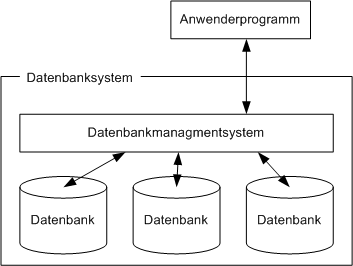
\includegraphics[width=4.16667in,height=\textheight,keepaspectratio]{datenbanksystem.png}

\subsubsection{10. Vorteile eines DBS}\label{vorteile-eines-dbs}

\begin{itemize}
\item
  Mehrfachnutzung der Daten. Dateninseln, in denen einzelne Benutzer
  ihre Daten isoliert verwalten werden vermieden. Somit kann Redundanz
  der Daten ausgeschlossen werden und eine Standardisierung der
  Datenformate erreicht werden.
\item
  Unabhängigkeit von Programmen und Daten. Programme kommunizieren mit
  der DB über vom DBMS angebotene Interfaces; Änderungen in den
  Strukturen der DB können vor den Programmen weitgehend verborgen
  werden.
\item
  Gewährleistete Datenintegrität. Das DBMS hat das Wissen über die
  Zustände der DB und kann Verletzungen der Integrität ausschließen.
\item
  Kontrollierter Mehrbenutzerbetrieb. Zeitlich überlappender Zugriff
  unterschiedlicher Programme zu gemeinsamen Daten kann durch das DBMS
  kontrolliert werden.
\item
  Datenpersistenz. Hardware- und Softwarefehler im laufenden Betrieb
  können repariert werden; das DBMS verwaltet selbst die hierzu
  erforderlichen Informationen.
\item
  Datensichten. Unterschiedliche Benutzergruppen benötigen auf ihre
  Bedürfnisse abgestimmte Sichten auf das zentrale konzeptuelle Schema.
  Das DBMS kann die erforderlichen Abbildungen zur Verfügung stellen.
\item
  Autorisierter Datenzugriff. Zugriff zu den Daten ist nur über das DBMS
  möglich. Damit kann nicht autorisierter Zugriff vermieden werden.
\item
  Komplexität. Die effiziente und sichere Nutzung im Rahmen kritischer
  praktischer Anwendungen erfordert speziell ausgebildetes Personal und
  verursacht erhebliche Hardware- und Software-Kosten. eingeschränkte
  Effizienz. DBS sind universelle Softwaresysteme, die für
  unterschiedlichste Arten von Anwendungen die geforderte Leistung zur
  Verfügung stellen wollen. Für spezielle Anwendungen kann ihre
  Leistungsfähigkeit deutlich geringer sein im Vergleich zu für diese
  Anwendungen spezialisierte Systeme. Aktuell kann man Diskussionen
  hierzu unter dem Stichwort ``NoSQL''verfolgen.
\end{itemize}




\end{document}
